\section{moeo\-Fitness\-Then\-Diversity\-Comparator$<$ MOEOT $>$ Class Template Reference}
\label{classmoeoFitnessThenDiversityComparator}\index{moeoFitnessThenDiversityComparator@{moeoFitnessThenDiversityComparator}}
Functor allowing to compare two solutions according to their fitness values, then according to their diversity values.  


{\tt \#include $<$moeo\-Fitness\-Then\-Diversity\-Comparator.h$>$}

Inheritance diagram for moeo\-Fitness\-Then\-Diversity\-Comparator$<$ MOEOT $>$::\begin{figure}[H]
\begin{center}
\leavevmode
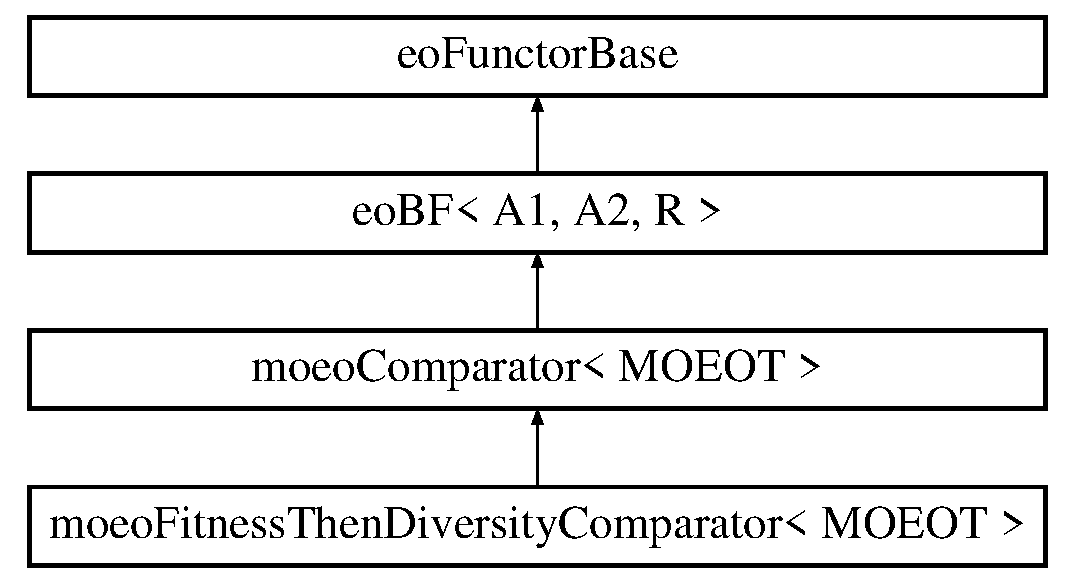
\includegraphics[height=4cm]{classmoeoFitnessThenDiversityComparator}
\end{center}
\end{figure}
\subsection*{Public Member Functions}
\begin{CompactItemize}
\item 
const bool \bf{operator()} (const MOEOT \&\_\-moeo1, const MOEOT \&\_\-moeo2)
\begin{CompactList}\small\item\em Returns true if \_\-moeo1 $<$ \_\-moeo2 according to their fitness values, then according to their diversity values. \item\end{CompactList}\end{CompactItemize}


\subsection{Detailed Description}
\subsubsection*{template$<$class MOEOT$>$ class moeo\-Fitness\-Then\-Diversity\-Comparator$<$ MOEOT $>$}

Functor allowing to compare two solutions according to their fitness values, then according to their diversity values. 



Definition at line 45 of file moeo\-Fitness\-Then\-Diversity\-Comparator.h.

\subsection{Member Function Documentation}
\index{moeoFitnessThenDiversityComparator@{moeo\-Fitness\-Then\-Diversity\-Comparator}!operator()@{operator()}}
\index{operator()@{operator()}!moeoFitnessThenDiversityComparator@{moeo\-Fitness\-Then\-Diversity\-Comparator}}
\subsubsection{\setlength{\rightskip}{0pt plus 5cm}template$<$class MOEOT$>$ const bool \bf{moeo\-Fitness\-Then\-Diversity\-Comparator}$<$ MOEOT $>$::operator() (const MOEOT \& {\em \_\-moeo1}, const MOEOT \& {\em \_\-moeo2})\hspace{0.3cm}{\tt  [inline]}}\label{classmoeoFitnessThenDiversityComparator_087856d1a7d81f242e95591d694e3ef6}


Returns true if \_\-moeo1 $<$ \_\-moeo2 according to their fitness values, then according to their diversity values. 

\begin{Desc}
\item[Parameters:]
\begin{description}
\item[{\em \_\-moeo1}]the first solution \item[{\em \_\-moeo2}]the second solution \end{description}
\end{Desc}


Definition at line 54 of file moeo\-Fitness\-Then\-Diversity\-Comparator.h.

The documentation for this class was generated from the following file:\begin{CompactItemize}
\item 
moeo\-Fitness\-Then\-Diversity\-Comparator.h\end{CompactItemize}
